\chapter*{The neuroanatomical signature of time in Working Memory}

% Il m'a fallu un temps conséquent pour me former au début du stage à l'analyse en EEG. 
% Au MVA, j'avais déjà fait des neurosciences, ainsi que la théorie physique des EEG et MEG à l'aide du cours d' \href{http://math.ens-paris-saclay.fr/version-francaise/formations/master-mva/contenus-/imagerie-fonctionnelle-cerebrale-et-interface-cerveau-machine-161979.kjsp?RH=1242430202531}{Imagerie fonctionnelle cérébrale et interface cerveau machine}, au cours duquel j'ai déjà manipulé les interfaces cerveau machines par exemple en
% \href{https://github.com/crsegerie/bci_competition}{réimplémentant} la solution des vainqueurs de la compétition \href{https://www.kaggle.com/c/inria-bci-challenge}{inria-bci-challenge}. Mais en réalité, lors de cette compétition kaggle, les participants ont été épargnés du préprocessing du traitement de la donnée des EEG : les organisateurs du kaggle avaient déjà nettoyé la donnée qui était alors utilisable par n'importe quel praticien en machine learning. Mais il existe tout un savoir faire afin de nettoyer la donnée, et ce nettoyage et cette analyse est presque plus technique que du machine learning conventionnel.



% \begin{comment}
% \section{Théorie}
% voir le cours de gramfort. Voir le cours du mva.
% \section{L'écosysteme MNE - Bids}
% \subsection{mne-python}
% \subsection{mne-bids-pipeline}
% \subsection{mne-bids}
% \end{comment}


\section*{Prelude}

I divided this report into two parts that roughly follow the chronological order of my internship.

The first chapter gives the scientific context of my internship. This part is an account of the environment in which I am inserted and of the knowledge required to understand my work hereafter. Scientific activity is no longer a solitary activity, especially in neuroscience, where the tools used are based on years of collective work. I notably explain in this chapter the ins and outs of the pilot study paper \cite{herbst2021abstracting} on which I rely. The goal of my internship is to complete this pilot study by analyzing magnetoencephalography (MEG) data, by finding appropriate mathematical methods to analyze the MEG data, and to implement these mathematical methods in an open source automatic analysis pipeline, the mne-bids-pipeline. This pipeline aims to allow future cognitive science researchers to analyze electroencephalogram data in a snap, while promoting replicability and open science. This part could constitute the introduction part of a future paper.

The second chapter presents the more technical aspects of my contribution to the reproduction of the pilot study. This replication using MEG imaging, I detail the method used to analyze the parts of the brain in action during the use of the working memory. We used the mne-bids-pipeline to analyze the data. But we had to adapt the mne-bids-pipeline by using new algorithms in order to meet the requirements of our experimental paradigm. An important part of my work has been allocated to implement in open-source these methods rigorously, while optimizing the computation time. This part could constitute the method, results of a future paper. The beginning of a discussion is also outlined.

\chapter{Scientific Context}

% Potentiellemnt dire : developper des methodes mathematiques qui vont permettre à la suite aux chercheurs d'utiliser la pipeline pour open sscience... Dire que nous avons pu égalemetn eu des premiers résultats afin de trouver les régions du cervaux, même si ce n'était pas le but premier de mon stge, une early analyse sous le prismes des sciences cognitive à été menée.

% This internship combines two aims: to extract the neural signatures of time stored in working memory from existing MEG data, and to contribute to ongoing efforts of establishing an open-science pipeline for MEG analysis in BIDS (standardized brain imaging data format, \cite{gorgolewski2016brain}). The project is part of a collaboration between NeuroSpin, and the MNE Python developers at Inria, with the aim to push the use of BIDS for more transparent and open MEEG research practices.

% As shown by a large number of studies, humans can perceive temporal intervals (durations in the range of seconds), judge or compare them with other intervals, and recognize or reproduce them later on. Hence, durations can be stored in memory, like sensory stimuli. It is however not known yet how the brain achieves this, for instance in which format (continuous or symbolic) durations are stored and which brain mechanisms support this ability \cite{polti2018effect}, \cite{teki2014working}. In this internship, I joined the inria/neurospin team in the ongoing analysis of the previously collected MEG data, with the aim to reconstruct source time courses of brain activity from the cortex, and possibly the hippocampus and cerebellum \cite{gauthier2020hippocampal} using volume source models in MNE-Python.

% The pipeline developed during the project will contribute to ongoing open-science
% efforts by the team to establish a robust and publicly available pipeline for source
% reconstruction of MEEG data based on the BIDS MEG data format in MNE-Python.


% Mes connaissances préalables: MVA cours imagerie fonctionnelel cerebrale + Neuroscience + imagerie médiacle


\section{The Time in Working Memory (TiWM) paradigm}

Cette partie présente the \textit{time in Working Memory} paradigm, qui a été exposé dans le papier \cite{herbst2021abstracting}. Le but de mon stage est d'aider à la reproduction de ce papier mais cette fois ci en utilisant des donnée venant de MEG.

\subsection{Description of the Pilot Study}

Planning for the future relies on the ability to remember the duration of events, but it is unknown how durations are stored in the brain's working memory.  The paper abstracting time in working memory proposes a new n-item delayed duration reproduction task to assess whether elapsed time is stored in memory as a continuous feature or as an abstract element. 

[present the clock models, but say that it is outside the spope of my internship. My training as a mathematician does not give me the tools to interpret the results, but simply through dialogue with the cognitive researchers, I propose mathematical methods].

The participants listened to sequences composed of empty time intervals that they had to reproduce as precisely as possible. For each sequence, one can manipulate the number of time intervals and the overall duration of the sequence to separate their effects on recall accuracy. The figure \ref{paradigm} presents the paradigm. Temporal reproduction accuracy decreased systematically with an increasing number of items. These results suggested that the number of time intervals, not their duration, determines recall precision. According to the brain clock models proposed by cognitive science, these results are interpreted as evidence of the existence of a symbolic representation of duration in working memory.



\begin{figure}[ht]
    \centering
    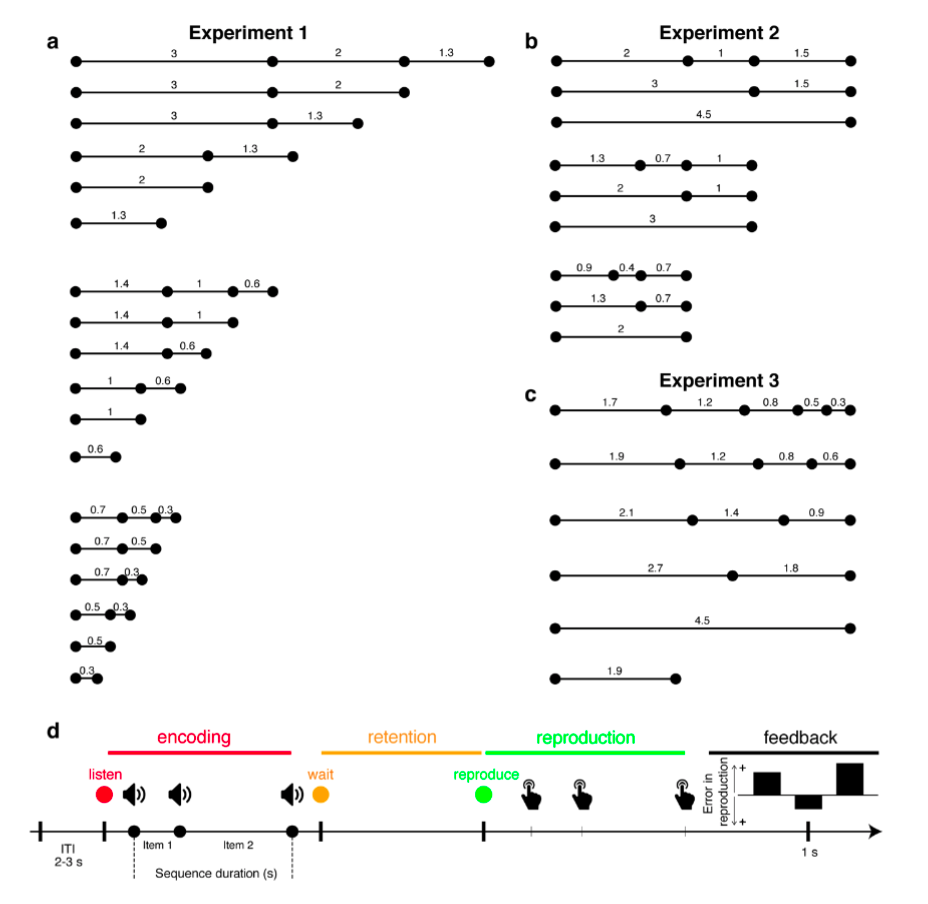
\includegraphics[width=10cm]{images_report/n-item delayed reproduction task.png}
    \caption[n-item delayed reproduction task]%
    {n-item delayed reproduction task - Panels a–c depict the individual items and sequences used in Experiment 1, 2, and 3, respectively. Black dots represent 1kHz tones. All numbers are durations in seconds. (a) The set of sequences used in Experiment 1, in which the number of items in a sequence and the full sequence duration covaried. A sequence was composed of 1, 2 or 3 items, and its duration varied from 0.3s to 6.3 s. \textbf{(b) In Experiment 2, the number of items and the sequence duration were orthogonalized. A sequence was composed of 1, 2 or 3 items with sequence duration fixed to 2 s, 3 s, or 4.5 s irrespective of the number of items composing it.} (c) In Experiment 3, a sequence was composed of 1 to 5 items. Only two sequence durations were used (1.9 s and 4.5 s). (d) Example trial. In all experiments, each trial was composed of four phases: First, participants listened to a sequence of pure tones demarcating time intervals of varying duration. Following a retention interval, participants were asked to reproduce the temporal sequence as precisely as possible. In the example depicted here, the sequence was composed of two items. Following the reproduction (green), feedback was provided showing the relative temporal reproduction error for teach item in the sequence.}

    \label{paradigm}
\end{figure}


\subsection{Goal of the internship: reproduce the pilot study using MEG data}

Thus, according to this first study, we know that durations are not represented in a continuous way, but in a symbolic way. But we still do not know in which part of the brain the information is stored. In order to visualize in which part of the brain the working memory is encoded, we reproduced the experiment this time by recording the cerebral data with magnetoencephalograms. In this new experiment, we no longer concentrate on the analysis of the accuracy of the restitution of the duration of the time intervals, but we will concentrate more on the visualization of the frequencies and cerebral areas at stake for the working memory.

Compared to the original study, we changed two main points:

\begin{itemize}
    \item We did not repeat the 3 experiments using MEGs, but only experiment 2, which orthogonalizes the number of items and the total sequence duration.
    \item In the original Experiment 2, three sequences durations were tested (2 s, 3 s and 4.5 s) and the number of items was 1, 2 or 3 items for each sequence. In our replication of this experiment, we use only sequences of either 1 or 3 items, which allows to maximize the effect size.
\end{itemize}

% - Les modèles de clocks cerebrales??
% - Pourquoi EEG plutot que FMRI


\subsection{Glossaire}

In the context of MEEG, the vocabulary used is very specific, and is essential to the understanding. The table \ref{Tab:Glossary_theory} gives the main vocabulary of the neural ocillation theory. The table \ref{Tab:Glossary_protocol} gives the usual vocabulary used in experimental protocols.

\begin{table}[ht]
    \centering
    \begin{tabular}{@{}| p{4cm}|p{9cm}| @{}}
        \hline
        EEG-MEG                     & The Electro-magnetoencephalography is a non-invasive methods for studying brain function that reflect the electrical activity of neuronal populations with millisecond temporal resolution.                                                                                                                                                             \\

        Local field potential (LFP) & electric potential in the extracellular space around neurons. LFP is a widely available signal in many recording configurations, ranging from single-electrode recordings to multi-electrode arrays                                                                                                                                                     \\
        Neuronal oscillations       & prominent feature of spontaneous and task-related brain activity that occur at the level of single units, local field potentials (LFPs), and EEG/MEG recordings. The traditional view is that neuronal oscillations reflect inhibition-based fluctuations of neuronal activity that emerge from the synchronous activation of large neuronal ensembles. \\
        Spectral power              & reflects the amplitude of neural oscillations computed through a time–frequency transformation (TFT).                                                                                                                                                                                                                                                   \\
        \hline
    \end{tabular}
    \caption{Glossary of the Neural Oscillation and of the Theory of the working memory. \cite{roux2014working}}
    \label{Tab:Glossary_theory}
\end{table}

\begin{table}[ht]

    \centering
    \begin{tabular}{@{}| p{3cm}|p{10cm}| @{}}
        \hline
        Session      & A logical grouping of neuroimaging and behavioural data collected consistently across participants. A session includes the time involved in completing all experimental tasks. This begins when a participant enters the research environment until he/she leaves it.                                                    \\
        Run          & An uninterrupted period of continuous data acquisition without operator involvement.                                                                                                                                                                                                                                     \\
        Event        & An isolated occurrence of a presented stimulus, or a subject response recorded during a task                                                                                                                                                                                                                             \\
        Epoch        & In the MEEG literature, the term epoch designates the outcome of a data segmentation process. Typically, epochs in event-related designs (for analysis of event related potentials or event related spectral perturbations) are time-locked to a particular event (such as a stimulus or a response)                     \\
        Evoked data  & Evoked objects typically store an EEG or MEG signal that has been averaged over multiple epochs, which is a common technique for estimating stimulus-evoked activity.                                                                                                                                                    \\
        Sensors      & Sensors are the physical objects or transducers that are used to perform the analogue recording, i.e., EEG electrodes and MEG magnetometers/ gradiometers. Sensors are connected to amplifiers, which not only amplify, but also filter the MEEG activity.                                                               \\
        Channels     & Channels refer to the digital signals that have been recorded by the amplifiers. It is thus important to distinguish them from sensors. A ‘bad channel’ refers to a channel that is producing a consistently artifactual or low-quality signal.                                                                          \\
        Sensor space & Sensor space refers to a representation of the MEEG data at the level of the original sensors, where each of the signals maps onto the spatial location of one of the sensors.                                                                                                                                           \\
        Source space & Source space refers to MEEG data reconstructed at the level of potential neural sources that presumably gave rise to the measured signals (according to an assumed biophysical model). Each signal maps onto a spatial location that is readily interpretable in relation to individual or template-based brain anatomy. \\
        \hline
    \end{tabular}
    \caption{Glossary of MEEG terminology commonly used to describe stimulation and task parameters and protocols as defined in \cite{pernet2018best}}

    \label{Tab:Glossary_protocol}
\end{table}



\section{EEG, MEG}

EEG and MEG measure the electrical activity of our brain using electrodes placed on the scalp. It tells us, from the surface measurements, how active the brain is. It is possible to measure both eeg and meg data, which is why the acronym meeg is used to designate these data.

For our experimental paradigm, it is much more important to have high temporal precession than high spatial precision. This is why we choose to use MEEG rather than fMRI to study this paradigm.

Indeed, the temporal sampling rate of MEG is high, with more than 1000 Hz per sencode. This high temporal resolution contrasts with that of functional magnetic resonance imaging, which essentially detects changes in the concentration of oxygen in the blood, a system with a much slower response in the human brain, with a lag of several seconds, and therefore not suitable for our temporal reproduction paradigm.


\subsection{MEG in comparison to EEG}

MEG is a cutting-edge functional brain imaging technology. MEG is extremely sensitive and measures very weak magnetic fields produced by the electromagnetic activity of neurons. MEG is the safest of the various brain imaging technologies: no energy is deposited in the individual being monitored. The machine does not even touch the head. MEG is particularly important in basic and clinical research and especially in studies with young child populations.

The advantage of measuring magnetic fields, rather than electric fields as in electroencephalography (EEG), is that they pass through the skull and other tissues between the active neurons and the MEG detectors without distortion, unlike EEG, where the signal is less accurate.

\subsection{Equipment: MEG in Neurospin}

MEGs are extremely rare in France, and MEG equipment in France can be counted on the fingers of one hand. But Neurospin is one of them. Our center has a shielded chamber protecting a MEG recording device from electromagnetic noise.

The MEG at Neurospin is an Elekta Neuromag device. The MEG helmet consists of 102 sensors-triplets (1 triplet = 2 orthogonal planar gradiometers and 1 magnetometer). The MEG data I am manipulating during the internship are composed of 204 gradiometer channels and 102 magnetometer channels (Figure \ref{raw_data}) This organization between gradiometer and magnetometer will be important when we try to speed up the algorithms in the section \ref{Sec:running_time_optimisation}

\begin{figure}[ht]
    \centering
    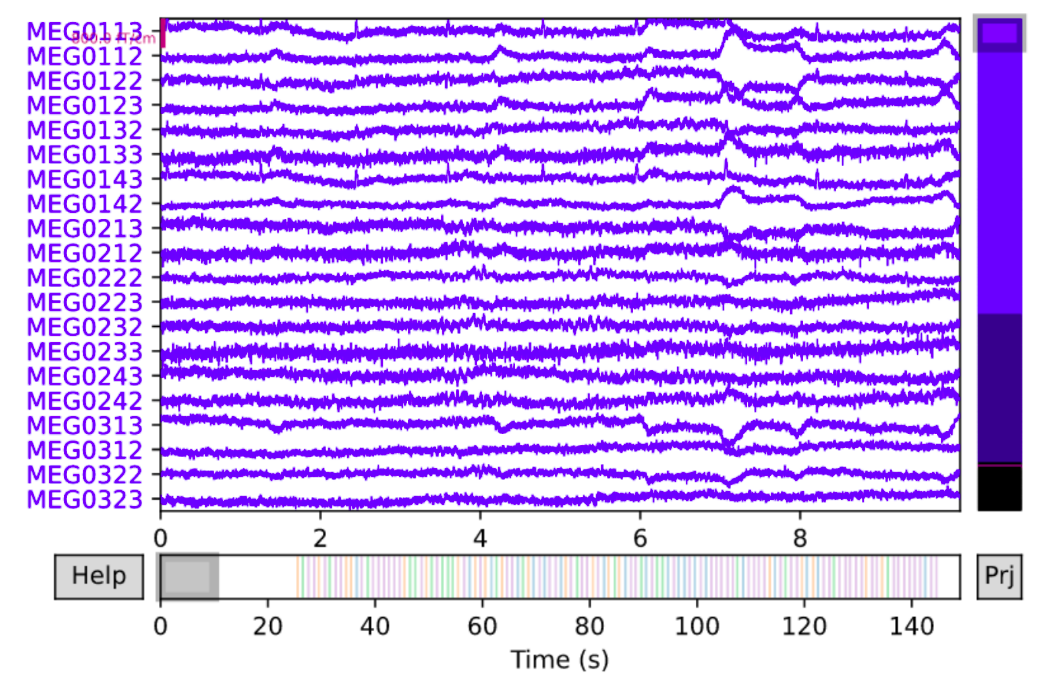
\includegraphics[width=10cm]{images_report/preprocessing/raw_data/Example_of_MEG_recording_reduced.png}
    \caption{Example of an MEG recording of a passive session. Here 20 of the 306 channels are represented.}
    \label{raw_data}
\end{figure}

\subsection{Frequency band}


The high temporal accuracy of MEG data allows the study of signals in the frequency domain. The main frequency bands used are defined in Table \ref{Tab:neural_freq_band}.

\begin{table}[ht]
    \caption{Comparison of EEG bands for a typical adult}
    \centering
    \begin{tabular}{@{}| p{1.2cm}|p{2.5cm}| p{4.5cm}|p{4.5cm}| @{}}
        \hline
        Band  & Frequency (Hz) & Location                                       & Normally                                                                \\
        Delta & $\leq  4$      & frontally in adults, high-amplitude waves      & slow-wave sleep                                                         \\
        Theta & 4–8            & Found in locations not related to task at hand & Drowsiness or idling. Associated with inhibition of elicited responses. \\
        Alpha & 8–14           & posterior regions of head                      & relaxed, inhibition control                                             \\
        Beta  & 14–30          & mainly frontaly, low-amplitude waves           & active thinking, focus                                                  \\
        Gamma & $\geq 30$      & Somatosensory cortex                           & Cross-modal sensory processing or short-term memory                     \\
        \hline
    \end{tabular}
    \label{Tab:neural_freq_band}
\end{table}


\section{The MNE ecosystem}

The MNE ecosystem is composed (among other things!) of three different libraries, nested by increasing dependency.

\begin{itemize}
    \item MNE-Python, which is an open-source Python package for exploring, visualizing, and analyzing human neurophysiological data mainly in EEG and MEG format. This library contains everything needed to manipulate EEG signals, from visualization to machine learning.
    \item MNE-BIDS. The Bids format is a convention for structuring MEEG datasets. MNE-BIDS is a library that facilitates the use of this convention in python.
    \item mne-bids-pipeline is a library allowing to automate the analysis of meeg data for datasets using the Bids format.
\end{itemize}

\subsection{MNE-Python}

MNE-Python \cite{GramfortEtAl2013a} is an open-source python library allowing to analyze brain data from EEG or MEG. The figure \ref{workflow_mne} allows to visualize the flow of the data from the collection of the anatomical information (T1) and the raw data collected by MEEG to the estimation of the tridimensional Sources.

For the comprehension of this report, the most important steps are on the left of the figure:

\begin{itemize}
    \item Raw data: The recording of the data is done in a continuous way during runs of 10 minutes. The recording is not stopped during this period. A run is composed of about 30 events.
    \item The data is pre-processed: defective sensors are removed, a low-pass filter is applied to keep only the useful brain signals, and an artifact removal technique such as ICA is used. The artifact rejection pipeline is presented in section \ref{preprocessing_of_artifacts}. 
    % [nested]
    \item Epoch data : After cleaning the run, we split the run into different events. In our study, the events are either composed by intervals of 3 items or intervals of one item.
    \item Evoked data : We average the events in order to obtain exploitable results. In our case we mainly calculate two averages, one for each number of items.
    \item Source Estimate. All the previous steps are carried out in the sensor space, that is to say in the space of the 306 sensors of the MEG, which represent 306 temporal series. The calculation of the source estimate allows to convert these temporal series into a 3D or 4D representation.
\end{itemize}

\begin{figure}[ht]
    \centering
    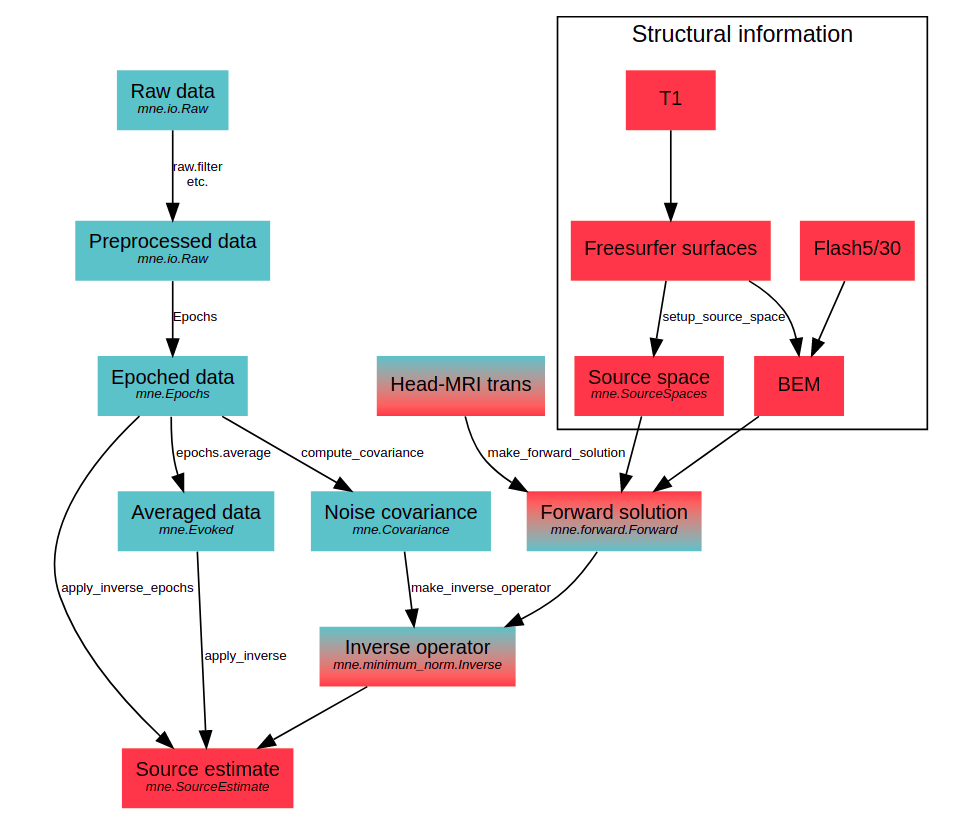
\includegraphics[width=13cm]{images_report/workflow_of_the_mne_software.png}
    \caption[Workflow of the MNE software]%
    {Workflow of the MNE software \cite{GramfortEtAl2013a}}
    \label{workflow_mne}
\end{figure}


\subsection{the Brain Imaging Data Structure (BIDS) format}

\begin{figure}[ht]
    \centering
    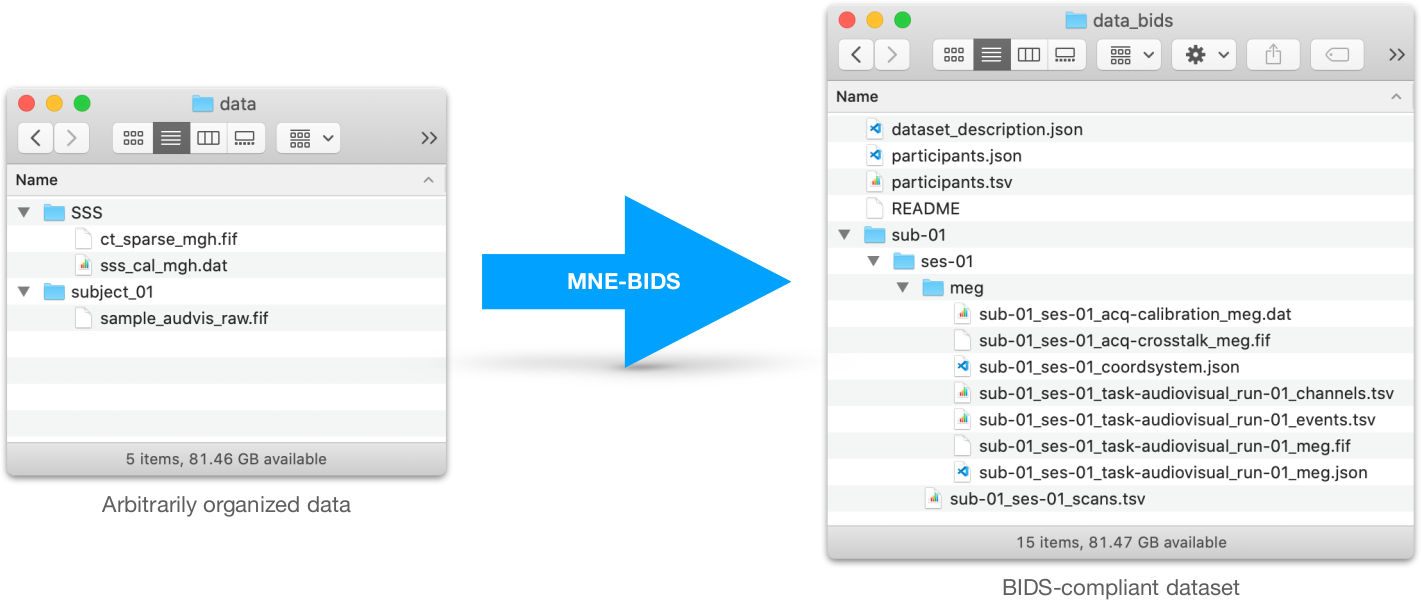
\includegraphics[width=10cm]{images_report/BIDS.png}
    \caption{An example of the use of the BIDS format.}
    \label{BIDS}
\end{figure}

\begin{figure}[ht]
    \centering
    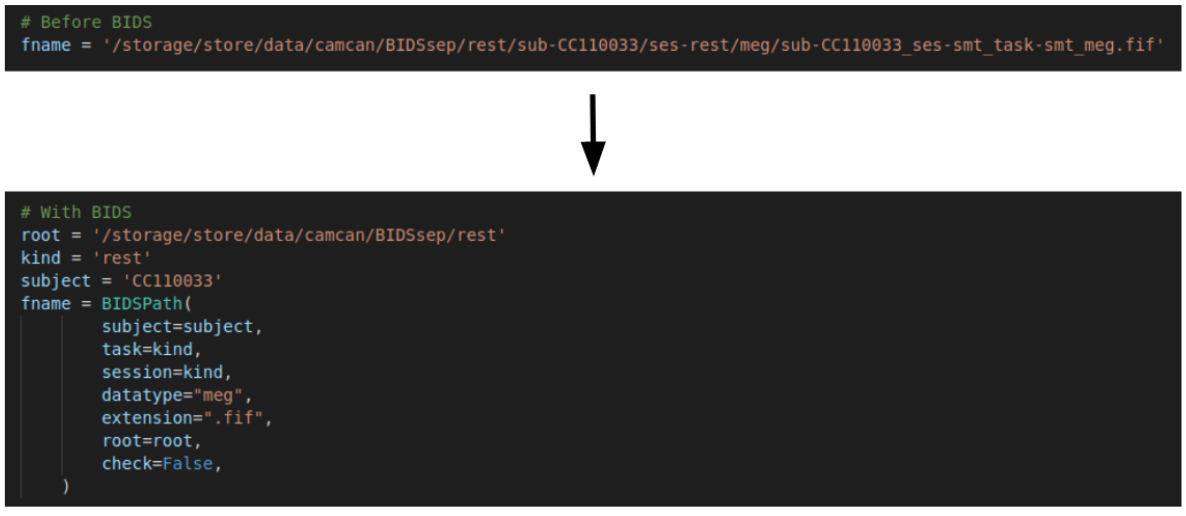
\includegraphics[width=10cm]{images_report/bids_example.png}
    \caption[Example of use of mne-bids]%
    {Example of the use of mne-bids in Python: we transform the initial long path into a modular function.}
    \label{bids_example}
\end{figure}

The brain imaging data structure was created to provide a simple way to organize neuroimaging data. The goal of this structure is to be a standard format to make the data accessible to everyone and avoid confusion. Using a Python package called MNE-BIDS \cite{appelhoff2019mne}, datasets can easily be converted to BIDS format. Datasets in BIDS format are supported by many tools. BIDS is the result of a collaborative effort to standardize brain data for easy analysis and sharing.

Figure \ref{BIDS} gives an example of a file architeture in BIDS format. Figure \ref{bids_example} shows an example of the use in python of the MNE-BIDS library. In the absence of a standard format, to access a file, the full path must be written. A path is specific to a file, so if you want to access another file or even another dataset, you will have to change the full path. If the dataset is in BIDS format, it is possible to use the BIDSPath function of MNE-BIDS to call a file. In this case, if you want to call another file or another BIDS-compatible dataset, you only need to change a few arguments of this function, such as the subject name or the root of the file, without having to worry about the full path, which makes it much more modular.

Thus, by implementing the BIDS format support, it is possible to switch from one BIDS-compatible dataset to another in the blink of an eye by changing only a few elements of the scripts.

\subsection{Automatic preprocessing with the MNE-BIDS-Pipeline}

Using BIDS-compatible datasets enables us to apply the MNE-BIDS-Pipeline to the preprocessing part of the model. The MNE-BIDS-Pipeline is an automatic preprocessing and processing pipeline for MEG and EEG data stored following the BIDS format \cite{gorgolewski2016brain}. To apply the preprocessing steps wanted, the MNE-BIDS-Pipeline only requires to set the corresponding parameter in a configuration file. Once it is done for one dataset it can be used on other datasets just by changing one line in the configuration file.

The MNE-BIDS-Pipeline (\url{https://github.com/mne-tools/mne-bids-pipeline}) is still in development. As I wanted to use it for the time in working memory paradigm, I had to help implement the missing features I needed.

The list of features to which I contributed is presented in the table \ref{Tab:PR}.

\begin{table}[ht]
    \centering
    \begin{tabular}{@{}| p{3cm}|p{9cm}| @{}}
        \hline
        Type & Title \\
        \hline
New feature & Add possibility to exclude runs from the analysis via the new exclude run setting. \\
Code health & Files docstrings in the preprocessing steps were updated. \\
Behavior changes & Warn if using ICA and no EOG- or ECG-related ICs were detected. \\
New feature & Added the possibility to have different runs for different subjects. \\
Behavior changes & Check that the baseline interval falls into the epoch interval. \\
Behavior changes & ica\_reject now also applies to ECG and EOG epochs. \\
Bug fix & The sanity check comparing the rank of the experimental data and the rank of the empty-room after Maxwell-filtering did not use the maxfiltered data. \\
Bug fix & epochs\_tmin and epochs\_tmax were named incorrectly in some test config files. \\
Bug fix & We now reject bad epochs by using ica\_reject before producing the "overlay" plots that show the evoked data before and after ICA cleaning in the `proc-ica\_report`. \\
New feature & It is now possible to analyze the contrast using the Common Spatial Patterns in the time-frequency domain using the new script: 03b-time\_frequency\_csp.py. We also test the significance of the contrast between the two conditions using cluster permutation statistics. \\
        \hline
    \end{tabular}
    
    \caption[Summary of my contributions to the MNE-BIDS-Pipeline.]%
    {Summary of my contributions to the MNE-BIDS-Pipeline on \href{https://raw.githubusercontent.com/mne-tools/mne-bids-pipeline/main/docs/source/changes.md}{GitHub}.}
    \label{Tab:PR}
\end{table}

It is very useful to employ this pipeline for the following reasons:
\begin{itemize}
    \item It improves reproducibility, as a simple setup file is now all that is needed to reproduce each figure.
    \item The pre-processing and analysis steps of MEEG studies are common to most studies, and only one or two scripts need to be modified (or created in our case) to obtain a complete study.
    \item Many of the meta parameters are hard to calibrate, especially for cleaning and when going through the source space. Without expertise, it is better to use the default parameters used in the pipeline.
    \item The pipeline allows to process the different participants in parallel, which allows to considerably accelerate the calculation times.
\end{itemize}
